\graphicspath{{../01Introduction/pics/}}

\chapter{Introduction}\label{ch:Introduction}

\begin{quoting}
	This quantum business is so incredibly important and difficult that everyone should busy himself with it. 
	
	
	A. Einstein in a letter to his friend Jakob Laub in 1908, as quoted by A. Wheeler in “The Mystery and The Message Of The Quantum”
\end{quoting}

{\bf Abstract}\hspace{0.2cm} In this chapter.


\lettrine[lines=2]{\color{darkocre}Q}{uantum physics is a century-old branch of physics. Its success} is unparalleled and yet quantum physics is unfinished in one sense: There is no clear and widely adopted consensus on what some of quantum ideas "really mean."

\section{What Is Quantum Physics?}
There are many characterizations of quantum physics.  In essence, quantum physics is the part of physics which focuses on \emph{quantum systems} -- physical systems showing \emph{quantum behavior}. So, what effects or phenomena are quantum and which ones are non-quantum (also called \emph{classical})?





\section{Who Needs Quantum Physics?}

Whether you want to contribute to the progress of science and technology, or just make sense of the most advanced knowledge of the world -- you will need familiarity with quantum physics. 

Modern technologies are based on a very broad range of physical phenomena described both by classical and quantum physics. Anyone doing research or working in applied science and engineering would benefit from solid understanding of physical concepts and laws. The importance of quantum physics has grown steadily over the past hundred years and it is clear now: The future is quantum. Today the knowledge and skills in quantum physics are key to success in such areas as quantum chemistry, laser physics, and quantum cryptography, to name a few.

The knowledge of quantum physics is also important to anyone trying to simply appreciate modern understanding of the world. Quantum physics is the best picture of the univeres we have today. However, the message of quantum physics is so unusual and often subtle, that understanding it properly requires a careful study instead of a cursory glance through a popular literature.


\section{Why is Quantum Physics Hard?}\label{sec:WhyQuantumHard}
Quantum physics is not an easy subject.  Mastering it requires learning new physical concepts and advanced mathematical tools. Additionally, it is necessary to examine critically some basic intuitive notions of classical physics and everyday experience.  All this takes time and effort.

\begin{mybio}{Feynman on Quantum Physics}
	In his book {\it The Meaning of It All}, Richard Feynman -- an American theoretical physicist and Nobel laureate -- wrote:
	
	
	"Trying to understand the way nature works involves a most terrible test of human
	reasoning ability. It involves subtle trickery, beautiful tightropes of logic on which one
	has to walk in order not to make a mistake in predicting what will happen. The quantum
	mechanical and the relativity ideas are examples of this."
	
	
	{\it The Meaning of It All, Section I: The Uncertainty of Science.}
\end{mybio}

Let us examine those features of quantum physics that make it particularly challenging and discuss what can be done to make the learning easier.

\subsection{Indirect Experience}
Concepts of classical physics, especially when applied to macroscopic objects, can often be connected to our experiences. Velocity, heat, force, pressure, motion of projectiles, currents of fluids, propagation of sound and so on -- all can be felt, seen, or otherwise perceived by humans. In contast, \emph{we do not have a direct access to the quantum side of the world.}  There are no experiments where one can say "Here, look at this entanglement!" or "Hey, touch this quantum of action!", or "Listen carefully, that is the decoherence!"

\begin{analogy}
	Imagine you want to understand the life of inhabitants of extremely distant land. The environment and climate of that land makes it impossible for you to travel there and see everything with your own eyes. 
	
	Who knows, maybe they do not have such notions as "home", "road", "tomorrow", "force", and so on.
	
	Now, if by "understand" we mean "explain and predict the behavior of aliens in our own terms", then the task might be hopeless. However, if by "understand" we mean "develop new concepts that describe and predict the behavior of aliens" then we might have a chance. Of course, the new concepts might be very foreign to us, at first. But the more we use them -- the less our mind struggles.
\end{analogy}


The problem then becomes two-fold. First, we need give up our non-quantum intution. Remember, our intution and conceptual pictures are rooted in macroscopic reality. We interact with the latter using our macroscopic organs and instruments which are unable to capture subtle non-classical features of the world. 

Second, we need to develop new intution and set of "pictures"/models which would be adequate for quantum world. While doing so, we must be careful not to "contaminate" this new way of thinking with old concepts. 

\subsection{Abstract Mathematics}
The mathematics used in modern physics is becoming increasingly more abstract. It is the price to pay for the powerful and general tools which are indespensible for expressing most advanced results of physics, either  classical or quantum.

Quantum physics does not use any special mathematical methods which would make it more challenging than classical physics. Of course, a student learning quantum theory might struggle with the heavy use of operators, complex vectors,  Hilbert spaces, commutators, matrices and so on. The difficulty, however, is not due to the quantum nature of the subject, since nearly all these mathematical concepts and tools could be found in other -- non-quantum -- areas of mathematical physics.

\begin{mybio}{Alfred Whitehead on Abstract Mathematics}
	Nothing is more impressive than the fact that as mathematics withdrew increasingly into the upper regions of ever greater extremes of abstract thought, it returned back to earth with a corresponding growth of importance for the analysis of concrete fact. ...The paradox is now fully established that the utmost abstractions are the true weapons with which to control our thought of concrete fact
	
	{\it Mathematics as an Element in the History of Thought, Ch. 2, p. 46}
\end{mybio}

Surprisingly, current mathematical framework of quantum physics is the simplest possible. Quantum theory is \emph{linear}, meaning that it is based on the \emph{superposition principle} and uses the \emph{simplest} kinds of operators -- \emph{linear operators}. It must be noted that the linearity is not exclusive to quantum theory, as, for example,  classical electrodynamics is also a linear theory.


\subsection{Inadequate Language}
Perhaps the biggest barrier on the path to mastering quantum physics is... \emph{ordinary language}. It has developed to communicate everyday experiences and emotions, but subtle natural phenomena are far removed from either of those.

\begin{mybio}{Bertrand Russell On Ordinary Language}
Ordinary language is totally unsuited for expressing what physics really asserts, since the words of everyday life are not sufficiently abstract. Only mathematics and mathematical logic can say as little as the physicist means to say.

{\it The Scientific Outlook (1931)}
\end{mybio}

\begin{mybio}{Werner Heisenberg On Ordinary Language}
	It is not surprising that our language should be incapable of describing the processes occurring within the atoms, for, as has been remarked, it was invented to describe the experiences of daily life, and these consist only of processes involving exceedingly large numbers of atoms. Furthermore, it is very difficult to modify our language so that it will be able to describe these atomic processes, for words can only describe things of which we can form mental pictures, and this ability, too, is a result of daily experience.
	
	{\it Principle of Quantum Theory (1930), Introductory, p. 11}
\end{mybio}
 
To capture deep and nuanced laws of nature, we must use a language of adequate power, built with new words and symbols completely foreign to common intuition and simple mental pictures. In other words, the adequate language has to be \emph{abstract}, \emph{purposefully developed}, and most likely \emph{unintuitive} to an untrained mind.
 
\begin{remark}
	Constructing new languages is a standard task in the field of computer science. New languages are regularly proposed to better describe computational tasks in a specific domain. For example, a separate language exists for working with database requests.
	
	In this field, a \emph{domain specific language} is usually developed to address problems 
	
	A language is considered good if it does not allow constructing meaningless or harmful statements. For example, if a language allows definition of a set of sets which are not elements of themselves, the this language will be plagued with the famous Russell paradox.  
	
	Natural human language is notoriously bad for formulating precise and abstract results of science.
\end{remark}

\begin{myrem}{Particles}
	Particles are excitations of quantum fields. They correspond to irreducible unitary representations of Lorentz group. Fields are operator-valued vector functions defined over Minkowski space and transformed simply under the action of the Poincare group.
\end{myrem}
Learning this language is the key to success. 

\section{Quantum Versus Classical}
Quantum physics does what classical physics failed to do: It provides a consistent, relatively simple, and extremely powerful set of physical and mathematical tools that describe, explain, and predict behavior of subatomic, atomic, molecular, and even macroscopic phenomena.

To understand the limits of classical physics and the advantages of quantum, a solid understanding of both is required. Moreover, at time classical physics may appear decepticely similar to the quantum physics, since quite a lot of terminology, concepts, and mathematical tools are shared by two. 

So when do we have to use quantum physics? Is there a border -- and how sharp? -- between quantum and classical phenomena? What are the main differences between the classical and quantum physics? What are the similarities?

\begin{figure}[htbp]
  \centering
  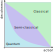
\includegraphics[scale=1.0]{quantumVsClassical}
  \caption{Physical processes exhibit quantum effects when either \emph{action} involved is on the order of 1-100 Planck constants or when \emph{quantum phase} is not washed out by \emph{decoherence} or both.}
  \label{fig:diagrams}
\end{figure}

\begin{mybio}{Semiclassical Physics}
	A set of methods have been developed to solve problems where the deviations from classical behavior was not too strong, but not negligible.  
\end{mybio}


\begin{mybio}{Correspondence Principle}
 	Quantum effects do not dissapear abruptly. The transition from quantum to classical behavior is, in certain sense, continuous. This opens a way to approach some problems of quantum physics with the knowledge of classical physics.   
\end{mybio}

\section{Quantum Enigma}
There are many adjectives that can be applied to quantum physics. It is tremendously successful, impactful,  fascinating, and intellectually rewarding. It also seems mysterous and "least understood" part of physics.

\begin{mybio}{What is Quantum Mechanics?}
	In 1968 in a German town Lindau, 480 young scientists met with 20 Nobel Laureates in Physics  -- the founders and major contributors to quantum physics. By this time the theory of quantum physics was fully formulated and applied to many important problems. One of the paticipating Nobel Laureates -- Willis E. Lamb Jr -- wrote:
	
	"A remarkable feature of the 1968 conference of Nobel prize winners in physics at Lindau is that it was possible for me to ask such question in the presence of two of the founders of quantuam mechancis, Werner Heisenberg and P. A. M. Dirac, more than 30 years after the discovery, in a lecture attended by 400 students who had recently begun their study of the subject." 
\end{mybio}

By 1968 most foundational papers and  many great textbooks on quantum physics had been written, including the books by Dirac and Heisenberg. Didn't those works define what quantum mechanics was?

By now quantum physics has demonstrated even greater success, but the questions like "What is Quantum Mechanics?" are still routinely raised in many books and articles. We are still puzzled by this enigmatic omni-tool that we discovered.

\begin{mybio}{Frank Wilczek on Quantum Theory}
	Frank Wilczek, an American theoretical physicist, received his Nobel prize in 2004 "for the discovery of asymptotic freedom in the theory of the strong interaction".
	
	In a paper {\it What Is Quantum Theory?}, published in Physics Today, he wrote:
	"To summarize, I feel that after seventy-five years -- and innumerable successful applications -- we are still two big steps away from understanding quantum theory properly."
\end{mybio}


\begin{figure}[htbp]
  \centering
  
\includegraphics[scale=1.0]{defaultFigureTemplate}
  \caption{Schematics can be used to represent functions, operators,
    their compositions and structure.}
  \label{fig:schematicExample}
\end{figure}


\section{Brief Historical Context}
The year 1900 is usually considered the birth year of quantum physics. On December 14 of 1900, at the meeting ????, the German physicist Max Karl Ernst Ludwig Planck presented his theoretical explanation of the \emph{spectrum} of electromagnetic radiation emitted by hot bodies. In his work he introduced what is now known as \emph{Planck's constant}  $h$, which has a physical meaning of \emph{elementary quantum of action}.
\begin{mybio}{Niels Bohr On $h$}
	The Danish physicist Niels Bohr, one of the founders of quantum physics, wrote: 
	
	\emph{
		"A new epoch in physical science was inaugurated, however, by Planck’s discovery of the elementary quantum of action, which revealed a feature of wholeness inherent in atomic processes, going far beyond the ancient idea of the limited divisibility of matter."
	}
	
	(Atomics Physics and Human Knowledge, Quantum Physics and Philosopy, Complimentarity and Causality.)
\end{mybio}
Let's take a look at what happened before and after Planck's discovery.

\subsubsection*{Pre-History: Spectroscopy and Molecular Theory}
The evolution of physics in the century preceding quantum era is fascinating. It is important to know some of pre-history in order to appreciate the context in which quantum physics was born. We will highlight two big advancements, one in experimental, and the other in theoretical departments. 

\subsubsection*{Spectroscopy}
First, the methods of \emph{spectroscopy}--study of energy distribution across various wavelengths of visible and invisible light--experienced significant development. Already in 1802 an English chemist and physicist William Hyde Wollaston observed that\footnote{Wollaston William Hyde 1802 XII. \emph{A method of examining refractive and dispersive powers, by prismatic reflection}, Phil. Trans. R. Soc. {\bf 92}: 365–380 } "If a beam of day-light be admitted into a dark room by a crevice 1/20 of inch broad\footnote{1/20 in = 1.27 mm.}, and received by the eye at the distance of 10 or 12 feet\footnote{10-12 feet = 3-3.7 m.}, through a prism of flint glass" one can see four colors (red, yellowish green, blue, and violet) separated by \emph{dark lines}. Soon many more dark lines in the optical spectrum of the Sun were discovered and systematically studied by a German physicist Joseph Ritter von Fraunhofer. Today these \emph{Fraunhofer lines} are understood to result from the \emph{absorption} of radiation by different atoms in the atmospheres of the Sun and earth.
\begin{figure}[htbp]
	\centering
	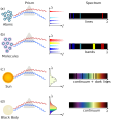
\includegraphics[scale=1.0]{spectraTypes}
	\caption{Various types of spectra observed from different substances. (a); (b); (c); (d). See text for explanation.}
	\label{fig:spectraTypes}
\end{figure}


The energy absorbed by a substance can be \emph{emitted}. The study of \emph{emission spectra} from various bodies revealed a great deal of complexity and provided a lot of information about bodies' material composition and state. 

There are four basic types of spectra one can observe, as illustrated in Figure \ref{fig:spectraTypes}. In a typical spectroscopic observation radiation from an excited object is sent through a \emph{dispersive} component, such as a prism or a diffraction grating\footnote{See Visual Glossary}. A beam of radiation is spread out according to colors and light of different color falls at different place of a detector (eye, photographic plate, or an electronic camera).

Light emitted by atoms consists of very definite colors which show up as \emph{emission lines} in spectra, as shown in Figure \ref{fig:spectraTypes}(a). Exact locations of such lines tell which atom emits the radiation. Simpler atoms, such as hydrogen or helium, have simpler spectra.

Spectra of excited molecules contain many closely placed lines. Sometimes multiple lines coalesce into a \emph{band}, as in Figure \ref{fig:spectraTypes}(b).

Radiation from large hot bodies, like Sun, reveals both discrete and continuous color distribution; see Figure \ref{fig:spectraTypes}(c). All colors are present in the spectrum, and dark Fraunhofer lines indicate that some of the radiation has been absorbed on its way to the detector by atoms and molecules.

Finally, an important radiation type corresponds to an \emph{idealized} object, called \emph{black body} -- a theoretical material which does not relfect any incident radiation. In other words, \emph{black body absorbs all incoming radiation}. Of course, black body also emits radiation, otherwise it would never stop accumulating energy from incident light. Therefore, black body \emph{is not truly black}, its perceived color depends on the temperature of the body. Emission spectrum of black-body, called \emph{black body radiation} or \emph{normal spectrum}, is of great interest, because it approximates emission spectrum from \emph{any material} kept at a constant temperature.
At the end of the 19th century, black body radiation was actively studied both experimentally and theoretically. 

\begin{mybio}{Max Planck And Black Body Radiation}
	Since black-body radiation spectrum does not depend on particular material, it has a universal nature. This fascinated Max Planck, as he wrote in his Scientific Autobiography\footnote{Max Planck, \emph{Scientific Autobiography and Other Papers}, Williams \& Norgate, 1950, pp. 34-35.}:
	
	\emph{"Thus, this so-called Normal Spectral Energy Distribution represents something absolute, and since I had always regarded the search for the absolute as the lofties goal of all scientific activity, I eagerly set to work."}
	
	\[
	\frac{\delta E}{\delta \nu} \propto \frac{\nu^3}{e^{a\nu}-1}\,,\,\quad a = h/kT\,.
	\]
\end{mybio}

The spectrum of black body radiation was the first type of spectrum to receive a theoretical explanation and an explicit formula. Spectra of atoms and molecules were properly studied only after the development of quantum mechanics.

Spectroscopy of the 19th century\footnote{William McGucken, \emph{Nineteenth-Century Spectroscopy}, The Johns Hopkins Press, 1969.}

\subsubsection*{Molecular Theory}
Second advancement of pre-quantum physics was connected with the hypothesis of atoms and molecules. Although atomistic ideas had been known for about two millenia, even in the 19th century far from every physicist was convinced that atoms and molecules were objects just as real as everyday things. There was no \emph{direct evidence} for the existence of atoms and molecules, and the main support for the atomistic views came from \emph{indirect evidence}, like the many useful results that followed from molecular theory. For example, the behavior of gases (diffusion, viscosity, laws connecting pressure and temperature, heat capacity, etc.) was especially well explained. Two major figures in this field were the Scottish physicis James Clerk Maxwell and the German physicist Ludwig Boltzmann.

In September of 1899, at the congress of the German Society of Natural Scientists and Physicians,  Ludwig Boltzmann presented a review titled \emph{"The Recent Development of Method In Theoretical Physics."}\footnote{\emph{The Monist}, January, 1901, Vol. {\bf 11}, No. 2, pp. 226-257.} He highlighted the rapid development of physics in the 19th century and discussed major experimental and theoretical results.

\begin{mybio}{Boltzmann's Prediction}
	\emph{"I have to mention finally the relations which obtain according to the molecular theory between the principle of entropy and the calculus of probabilies, concerning the real significance of which there may be some difference of opinion, but which, no unprejudiced person will deny, are eminently qualify to extend our intellectual horizon and to suggest new combinations both of ideas and experiments."}
\end{mybio}
Boltzmann's anticipation that "the principle of entropy and the calculus of probabilities" will lead to "new combinations both of ideas and experiments" was fully confirmed by Max Planck in about a year!

As explained in the Section XX, Max Planck used nearly the same approach as Boltzmann to calculate entropy of a thermodynamic system. Only in his case, the system was not an ideal gas of molecules, but a collection of oscillating molecules that interact with electromagnetic radiation (in the form of heat).

\subsection{1935 And 1965}
The experimental and theoretical quantum physics were advancing fast. There were many milestones, two of which we would like to highlight, as they are strongly connected to the modern issues of quantum physics, technology, and even philosophy.

\subsubsection*{EPR Paper}
In March of 1935 a paper titled \emph{"Can Quantum-Mechanical Description of Physical Reality Be Considered Complete"} was published, authored by Albert Einstein, Nathan Rosen, and Boris Podolsky. The work is known as \emph{EPR paper}, and the issue raised  in it is sometimes referred to as \emph{EPR paradox}.

\subsubsection*{Schrodinger Cat}
EPR paper stirred the community and prompted a couple of replies. Erwin Schrodinger wrote a paper \emph{"The Current State of Quantum Theory"} (???)  where he analyzed the EPR problem. He also introduced the concept of \emph{entanglement} and now famous "dead-and-alive" cat.

\subsubsection*{Bohr Dense Paper}
Niels Bohr -- a giant of quantum physics -- also replied to EPR paper in October of 1935. His main criticism was focused on how EPR group defined \emph{physical reality}. 

Bohr's reply is not an easy read.

\subsubsection*{Bell's Theorem}
The debates about the intricacies of quantum theory never faded. But in 1965 they were taken to a new level, by John Stewart Bell, who proposed a way to \emph{empirically} distinguish two modes of thinking about reality. 

In essense, for the proposed experiment, classical physics predicted result $A$  while quantum physics predicted the result $B\ne A$. Experimental tests pointed towards $B$.


\subsection{Three Ages of Quantum}
The evolution of quantum science and technology can be roughly divided into three stages: (a) "Old quantum physics" (b) modern quantum physics, and (c) information-age quantum physics (see Figure \ref{fig:quantumTechnologyEvolution}). Each stage is defined by the type of quantum systems in the focus of research and technology. 

\begin{figure}[htbp]
	\centering
	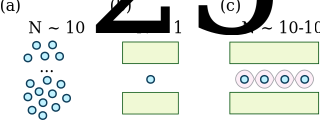
\includegraphics[scale=1.0]{quantumTechnologyEvolution}
	\caption{Three stages of quantum science and technology: (a) Observation of large groups of objects (atoms, molecules); (b) Study of interaction between single particles (one atom + one photon); (c) Connecting tens and hundreds of quantum systems using \emph{entanglement}.}
	\label{fig:quantumTechnologyEvolution}
\end{figure}


\subsubsection*{Old Quantum Physics}
Observations of early quantum phenomena, such as atomic spectra or photoeffect, involved  very large number of particles (atoms, photons, electrons; see Figure \ref{fig:quantumTechnologyEvolution}(a)). Addressing single particles seemed unrealistic in practice. This made the probabilistic nature of quantum theory even more similar to classical statistical mechanics.


\subsubsection*{Modern Quantum Physics}
A new age of quantum physics began when it became possible to study behavior and interaction between individual particles: atoms and field excitations (e.g. photons). A whole new field, called  cavity quantum electrodynamics (CQED) was born. Figure \ref{fig:quantumTechnologyEvolution}(b) shows a schematic of a cavity formed by two mirrors, with a single atom inside the cavity. During this era a number of beautiful experiments, demonstrating purely quantum effects which were previously discussed only theoretically, have been performed. 


\subsubsection*{Information Age}
The next step was studying quantum behavior and interaction of several particles (Figure \ref{fig:quantumTechnologyEvolution}(c)). 
The ability to produce and manipulate special \emph{multipartite quantum states} opened the doors into the age of \emph{quantum information science}. The role of \emph{entanglement} as a \emph{resource} for performing useful information processing tasks has been in the center of very active research.

The potential of quantum physics for sending and processing of information became apparent early. Quantum effects offer unique opportunities for secure communication and ultra-fast computation of certain algorithms. Despite many advances in these areas, the challenge is still great, especially in building a universal quantum computer.

\begin{mybio}{Slow Road to Quantum Computing}
	The idea of using quantum effects for computational task has been suggested by Richard Feynman in 1982 paper \emph{Simulating Physics with Computers}.
	
	In an interview with Google's Director of Quantum Algorithms Ryan Babbush, Columbia university professor and the host of the World Science Festival Brian Green asked\footnote{World Science Festival talk {\it What They Rarely Reveal About Quantum Computing: Without an Algorithm, It's Hype}. Available online.}:
	"What is the largest composite number that has been factored today with a quantum computer? " To which Ryan answered: "Oh, not a large one. [...]  Something like 15 or 25 or something." 	 
\end{mybio}

The challenge is to create and maintain entanglement of a larger number of quantum systems. 
"In summary, in the span of less than two decades, photonic quantum information science has matured immensely. [...]. The number of photons simultaneously used in experiments has grown, from 2 to 4 up to 12"
(Appl. Phys. Rev. 6, 041303 (2019))

\vspace{1cm}
\section*{Chapter Highlights}
{\setstretch{1.5}\chhc
  \it
\begin{itemize}
\item Natural evolution of mathematical objects from numbers, through
  vectors, leads to tensors.
\item Each successive tier of mathematical object in the progression
  ``numbers, vectors, tensors''  is more abstract and more powerful.
\item Numbers, vectors, and tensors are all conceptually connected.
\end{itemize}
}
